\icode{E-MI-SI-L2-261108-002}
如图是石桥正中央一孔，位于中央的楔形石块1，左侧面与竖直方向的夹角为\(\theta\)，右侧面竖直。若接触面间的摩擦力忽略不计，则石块1左、右两侧面所受弹力的比值为\paren[]

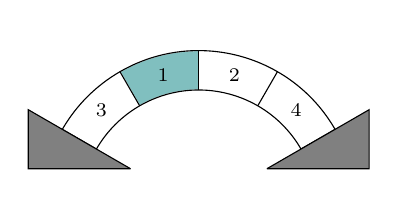
\begin{tikzpicture}[font=\scriptsize]
	\draw[fill=teal!50,draw=white] (120:1.5)--(120:2)arc(120:90:2)--(90:1.5) arc(90:120:1.5);
	\foreach \d in {30,60,...,150}
		\draw (\d:1.5)--(\d:2);
	\draw (30:1.5) arc(30:150:1.5);
	\draw (30:2) arc(30:150:2);
	\draw[fill=gray] (30:1)--(30:2.5)|-(30:1);
	\draw[fill=gray] (150:1)--(150:2.5)|-(150:1);
	\foreach \d/\n in {45/4,75/2,105/1,135/3}
		\node at(\d:1.75){\(\n\)};
\end{tikzpicture}
\begin{choices}
	\item\(\dfrac{1}{\tan\theta}\)
	\item\(\sin\theta\)
	\item\(\dfrac{1}{\cos\theta}\)
	\item\(\dfrac{1}{2\cos\theta}\)
\end{choices}
\begin{answer}
	C\qquad 提示：分解力，合成力。
\end{answer}